\subsubsection{Termination}

In this section we describe the termination algorithm designed for the
application.
During the description we will consider the IL as
split in two adjacent stacks:

\begin{itemize}
  \item upward stack: these components forward the messages
  from middleware to the application layer;
  \item downward stack: these components forward the messages
  from application layer to the middleware.
\end{itemize}

The termination order is
given by the path taken by the shutdown message
(Figure \ref{fig:termination-app}).

\begin{figure}[H]
  \centering
  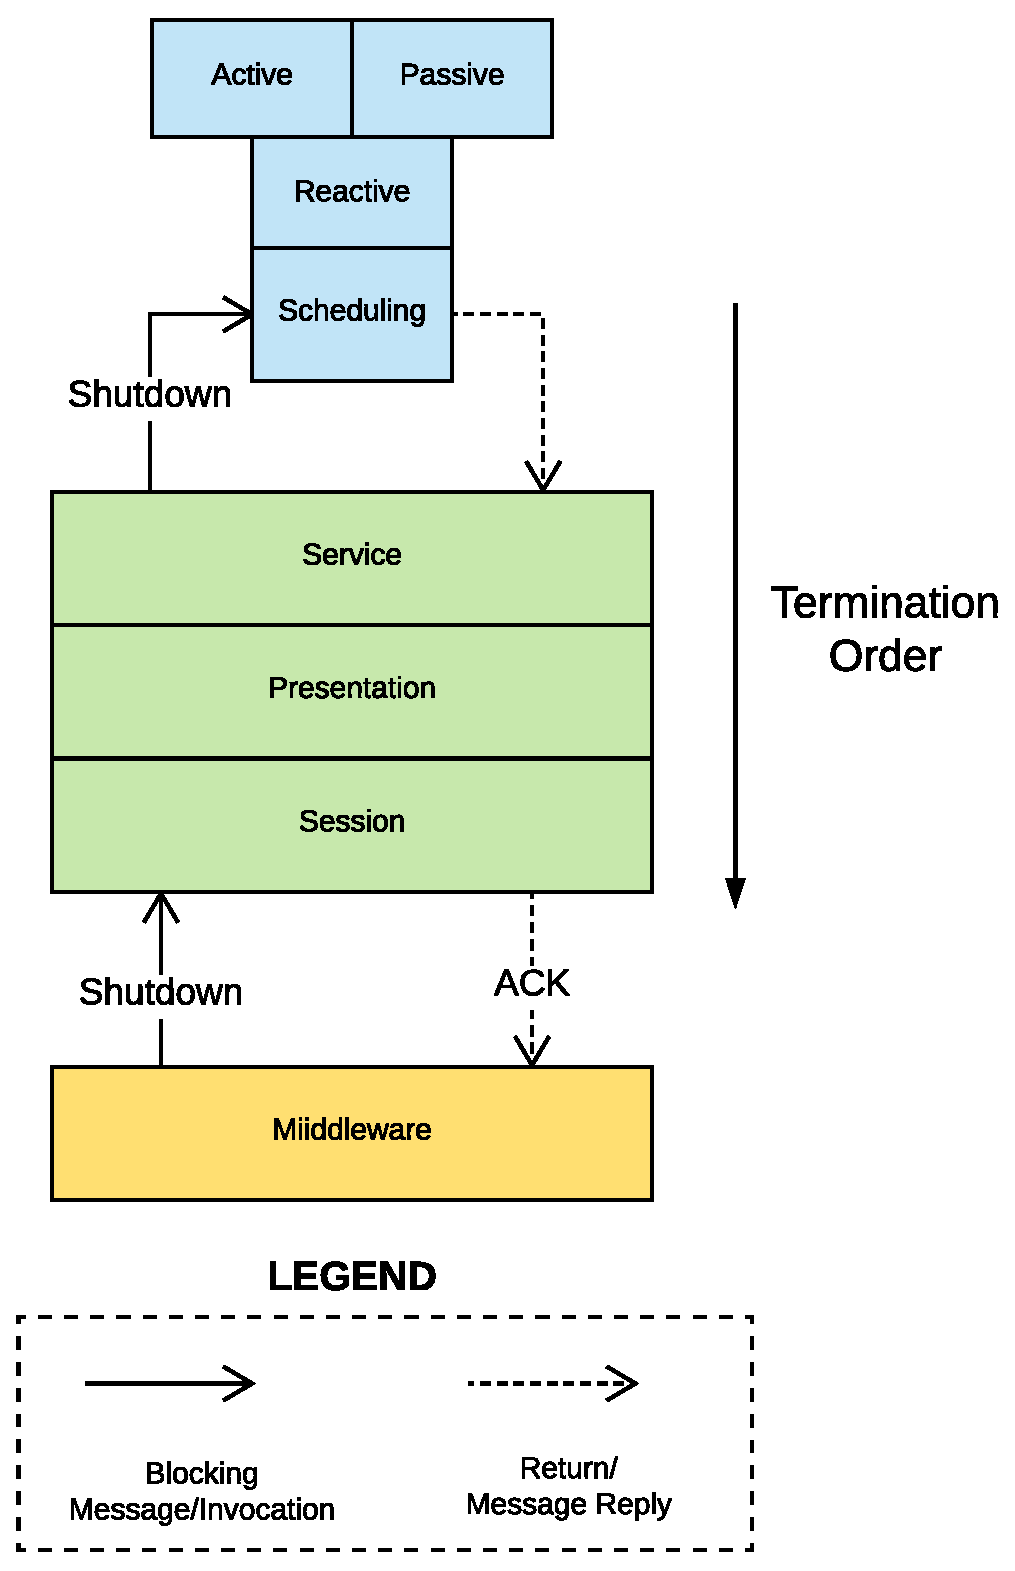
\includegraphics[scale=0.4,keepaspectratio]
    {images/solution/termination-app.eps}
  \caption{Application Termination}
  \label{fig:termination-app}
\end{figure}


The behavior of the backend is the following:


%TODO: Review termination process
\begin{enumerate}
  \item The middleware sends a \verb|shutdown| message to IL;
  \item The upwards components of IL terminate themselves when they
  read the shutdown request in the header. This is achieved by a transition
  from \verb|active| to \verb|stopped| state, which enables the master
  of each event loop to wait for all its workers to complete. Then the master
  puts the shutdown notification in the queue of the next IL component;
  \item The shutdown message is forwarded upwards until it reaches the Scheduling
  component. Then the scheduler notifies its workers. The workers change their
  state to \verb|stopped| and wait on a barrier until all the other workers have
  completed their execution. \\
  At this stage, we have the guarantee that no worker is running at
  the Application Layer level. Indeed, all the Application Layer
  entities are inerts because their engine (i.e., the scheduler) has been
  turned off;
  \item The previous point implies that we can safely terminate
  also the downwards components of the IL subsytem. Indeed, no message
  will be sent if the scheduler is not running. Thus, as last message,
  an acknowledgment to the shutdown request
  originally sent by the middleware is packed
  by the stub component and sent downwards through IL;
  \item All the downwards components of IL behaves exactly as the upwards one;
  \item The sender component forwards the acknowledgment message
  to the middleware and then shutdown itself.
\end{enumerate}


We implement also a dump method, to enable each stateful entity to save its
state before terminating. However we have not
been able to test this method in a distributed environment. Thus, we
kept it in the source code but without using it in production.


If the application layer crashes during the termination process, we eventually
guarantee the backend to complete its termination. Indeed, the
orchestrator should apply the restarting policy and reactivate the container;
allowing the middleware to check the successful termination.
However, we never experienced
such a failure neither been able to reproduce it with automated tests.


Similarly to the bootstrap phase, the middleware expects to receive the
\verb|shutdown| ack message within a certain amount of time.
In order to do so, when sending the message, the middleware starts a timeout.
Wherefore if it expires before receiving a response message,
it retransmits again the \verb|shutdown| request towards the application.
